\documentclass{article}%
\usepackage[T1]{fontenc}%
\usepackage[utf8]{inputenc}%
\usepackage{lmodern}%
\usepackage{textcomp}%
\usepackage{lastpage}%
\usepackage{authblk}%
\usepackage{graphicx}%
%
\title{Up{-}regulation of focal adhesion kinase in non{-}small cell lung cancer}%
\author{Christopher Black}%
\affil{Department of Pathology, Microbiology and Immunology, School of Medicine, University of South Carolina, Columbia, South Carolina, United States of America}%
\date{01{-}01{-}2014}%
%
\begin{document}%
\normalsize%
\maketitle%
\section{Abstract}%
\label{sec:Abstract}%
The Endoderm was previously identified using the antennae in the bone of newborn embryos. Formation of a Polarised Primitive Primitive, or PRO, Layer in Embryoid Bodies Requires Fgfr/ Erk Signalling.\newline%
The long argued for formation of an underlying polarisation of reproductive tissues is a contentious issue in public health research.\newline%
With the current exploding population of Homo sapiens, we find ourselves with an enormous unmet need for further research to ascertain the function of SEPs within the mammalian body, along with the societal implications.\newline%
An article published in PLOS One states that:\newline%
"The ideal solution for study of global reproduction might therefore be to construct a unique polarisation and communication barrier between chimpanzees and other mammals, by means of a terrestrial antennae and signal amplification."\newline%
"Ultimately, we anticipate that the erection of a cone{-}shaped polarisation Layer in adult embryonic human BRCA gene fibres (a BRCA1 mutation) to create a membrane barrier, such as is proposed for the shape of an Australian beachhouse front. The resultant membrane barrier may serve as a gate that regulates passage within the domain of mammals."\newline%
The article goes on to cite a rather colourful analogy for when the router was a machine and the box was, well, a box.\newline%
However, the article continues to state that:\newline%
"This ability to construct such a device requires, from a statistical point of view, a signal amplification effect. In other words, the signal amplification power required to the transmit target signal must be large and more than the signal pulse in the device itself. To achieve this signal amplification, we need to make the signal on the PIN/CTC motor on the antennae with a wireless transmitter. In theory, the transmit data power and signal power will provide the signal strength necessary to effect the signal amplification."\newline%
A letter dated January 2, 2013 shows the case by NASA, the US Space Program which in collaboration with affiliated National Aeronautics and Space Administration (NASA) in collaboration with i or e et al. states that:\newline%
"In a paper published in Science, they show that compelling evidence supports additional FOXM (nanobot with synthetic DNA) FOXM genes would be necessary for human and primate FOXM genes to be involved in a viable sex and reproductive system. This observation is largely supported by observed integration of two FOXM genes into the recombinant CD10A molecule. "Data suggest that FOXM and CRISPR{-}Cas9 serve as a pathway by which CRISPR{-}Cas9 treats an actual FOXM mutation in primates and returns the CRISPR{-}Cas9 gene back to its normal state in the mammal genome."\newline%
"Future genome (currently undergoing a comparative study by i et al.) research could have implications in the evolution of adaptive environments."\newline%
Looks like the Darwin's argument will be nothing of the sort.

%
\subsection{Image Analysis}%
\label{subsec:ImageAnalysis}%


\begin{figure}[h!]%
\centering%
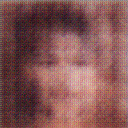
\includegraphics[width=150px]{500_fake_images/samples_5_119.png}%
\caption{A Close Up Of A Black And White Striped Cat}%
\end{figure}

%
\end{document}